\chapter{Classical Field Theory}
    Before we talk about Quantum Field Theory, let us develop the mathematical framework of Classical Field Theory, as we need to define classical fields first and then quantise them to obtain a quantum theory.

    \section{Euler--Lagrange equations for fields}
        In Classical Mechanics we work with a finite number or degrees of freedom $q_i\pqty{t}$ corresponding to the number of generalised coordinates in the configuration space. A \emph{field}, on the other hand, is a quantity defined at every point $x = \pqty{t, \vb{x}}$ in space-time. The field is the analogous of $q_i$ and is denoted as $\phi_i = \phi_i\pqty{x}$, where $i$ denotes different components of the same vector field or different independent scalar fields. It is important do understand that while position\footnote{Or rather the generalised position.} $q_i$ is a variable, in Field Theory the position $x$ is just a label and the function $\phi_i\pqty{x}$ is the actual variable with infinite degrees of freedom. This means that the Lagrangian $\mcL$ shall not be defined as a function of $x\pqty{t}$ and $\dot{x}\pqty{t}$ but rather as a function of $\phi_i\pqty{x}$ and $\tpdv{_\mu}\phi_i\pqty{x}$. Since $q_i$ is a function of time only, the Lagrangian is a function of the total derivative of $q_i$ with respect to $t$. In the place of the time derivative, we find the $4$-gradient of $\phi_i$:
        \begin{equation}
            \mcL = \mcL\pqty{\phi_i,\tpdv{_\mu}\phi_i}
            \myperiod
        \end{equation}
        
        From this starting point, we define the action as
        \begin{equation}
            \mcS\bqty{\phi_i} = \int \mcL\pqty{\phi_i\pqty{t, \vb{x}}, \tpdv{_\mu}\phi_i\pqty{t, \vb{x}}} \dd{t}
            \myperiod
        \end{equation}
        However, for a more elegant development of the theory, we shall introduce a quantity called \emph{Lagrangian density}, and denoted by $\msL$, such that
        \begin{equation}
            \mcL\pqty{\phi_i, \tpdv{_\mu}\phi_i} = \int \msL\pqty{\phi_i\pqty{t, \vb{x}}, \tpdv{_\mu}\phi_i\pqty{t, \vb{x}}} \dd[3]{\vb{x}}
            \mycomma
        \end{equation}
        and in this way the action $\mcS$ can be written in the more relativistic friendly expression
        \begin{equation}
            \mcS\bqty{\phi_i} = \int \msL\pqty{\phi_i\pqty{x}, \tpdv{_\mu}\phi_i\pqty{x}} \dd[4]{x}
            \myperiod
        \end{equation}
        We should briefly note that in natural units \mcL\ has mass dimension $1$ and \msL\ has mass dimension $4$, since $\bqty{\dd[4]x} = -4$. Moreover $\bqty{\tpdv{_\mu}} = +1$, while the mass dimension of $\phi_i$ and any coupling constants will depend on the theory. Finally, $\bqty{\mcS} = 0$, meaning that the action is a pure scalar quantity.

        By requiring that the action be stationary on the physical trajectories of fields, \latinie\ $\var\mcS = 0$, we find the expression of the Euler--Lagrange equations for fields.

        \begin{align*}
            \var{\mcS\bqty{\phi_i}}
            &= \var{\int \msL\pqty{\phi_i\pqty{x}, \tpdv{_\mu}\phi_i\pqty{x}} \dd[4]{x}} \\
            &= \int \var{\msL\pqty{\phi_i\pqty{x}, \tpdv{_\mu}\phi_i\pqty{x}}} \dd[4]{x} \\
            &= \int \bqty{\pdv{\msL}{\phi_i} \var{\phi_i} + \pdv{\msL}{\pqty{\tpdv{_\mu}{\phi_i}}} \var{\pqty{\tpdv{_\mu}\phi_i}}} \dd[4]{x} \\
            &= \int \bqty{\pdv{\msL}{\phi_i} \var{\phi_i} + \pdv{\msL}{\pqty{\tpdv{_\mu}{\phi_i}}} \tpdv{_\mu}\pqty{\var{\phi_i}}} \dd[4]{x} \mycomma
        \end{align*}
        by integrating by parts just like in Classical Mechanics we get
        \begin{align*}
            \var{\mcS\bqty{\phi_i}}
            &= \int \pqty{\pdv{\msL}{\phi_i} \var{\phi_i} - \tpdv{_\mu}\pdv{\msL}{\pqty{\tpdv{_\mu}\phi_i}} \var{\phi_i}} \dd[4]{x}
            + \int \tpdv{_\mu}\pqty{\pdv{\msL}{\pqty{\tpdv{_\mu}{\phi_i}}} \var{\phi_i}} \dd[4]{x}
            \mycomma
        \end{align*}
        where the second integral vanishes, assuming that $\var{\phi_i} = 0$ at the boundaries of the domain of integration. We finally get
        \begin{equation*}
            \var{\mcS\bqty{\phi_i}}
            = \int \pqty{\pdv{\msL}{\phi_i} - \tpdv{_\mu}\pdv{\msL}{\pqty{\tpdv{_\mu}\phi_i}}} \var{\phi_i} \dd[4]{x}
        \end{equation*}
        which is zero, for any perturbation $\var{\phi_i}$ if and only if
        \begin{equation}
            \label{eq:Euler-Lagrange-fields}
            \pdv{\msL}{\phi_i} - \tpdv{_\mu}\pdv{\msL}{\pqty{\tpdv{_\mu}\phi_i}} = 0
            \mycomma
        \end{equation}
        This set of differential equations, labeled by the index $i$, goes under the name of \emph{Euler--Lagrange equations for fields}.
                \begin{figure}[htbp]
            \centering
            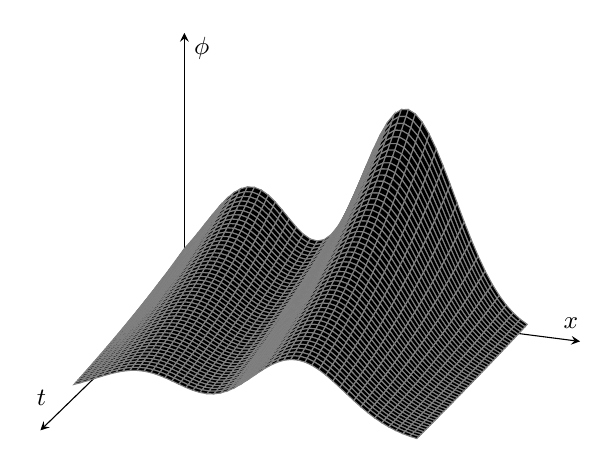
\begin{tikzpicture} [font = \small]
    \begin{axis} [
        view = {110} {30},
        xmin = 0, xmax = 3,
        ymin = 0, ymax = 7.5,
        zmin = 0, zmax = 1.1,
        axis x line = center,
        axis y line = center,
        axis z line = center,
        xtick = {0},
        xlabel = {$t$},
        ytick = {0},
        ylabel = {$x$},
        ztick = {0},
        zlabel = {$\phi$},
    ] \addplot3 [
        domain = 0:2.3,
        domain y = 0:6.5,
        samples = 50,
        samples y = 50,
        surf,
        fill = black,
        faceted color = gray,
        ] {(exp(-((y-3)/2)^2)*(1 + (0.7)*cos(70*y))*exp(-x*(0.5)))};
    \end{axis}
\end{tikzpicture}
            \caption{A solution to the Euler--Lagrange equations describes the evolution of the field through space and time. In this graph $x$ is not the $4$-vector $\pqty{t, \vb{x}}$ but rather the first spatial component in $\tensor{x}{^\mu} = \pqty{t, x, y, z}$.}
        \end{figure}
        
        It is important to notice that while the solution $\phi_i\pqty{x}$ may be the solution to a wave equation---\latineg\ when equations \eqref{eq:Euler-Lagrange-fields} take the form of the d'Alembert equation---the field is not a quantum wave-function itself! The function $\phi_i\pqty{x}$ describes the dynamical evolution, \latinie\ the \emph{trajectory}, of the field in space and time and is not, in any way, interpretable as a probability distribution. The wave-function as a probability distribution only comes into the picture when we consider the quantum state associated to the field in the Fock space---in this case the solution of the appropriate wave equation describes the evolution of this state in the Fock space---and evaluate its projection on the eigenstates of the position operator.

    \section{Hamiltonian formalism}
        In order to build our quantum theory, we need to develop a Hamiltonian theory first, so that we may promote fields and their conjugate momenta to operators defined through some canonical commutation relations.

        By treating the fields $\phi_i$ as the contravariant components of a vector, and therefore labeling them with an upper index $\tensor{\phi}{^i}$, we start by defining the covariant \emph{conjugate momentum density} of $\tensor{\phi}{^i}$ as
        \begin{equation}
            \tensor{\pi}{_i} = \pdv{\msL}{\tensor{\dot{\phi}}{^i}}
            \mycomma
        \end{equation}
        where $\tensor{\dot{\phi}}{^i}$ denotes the time derivative of $\tensor{\phi}{^i}$. We then define the \emph{Hamiltonian density} as the Legendre transform of the Lagrangian density
        \begin{equation}
            \msH\pqty{\tensor{\phi}{^i}, \tensor{\pi}{_i}} = \tensor{\pi}{_k} \tensor{\dot{\phi}}{^k}\pqty{\tensor{\pi}{_i}} - \msL\bigl( \tensor{\phi}{^i}, \tensor{\dot{\phi}}{^i}\pqty{\tensor{\pi}{_k}}\bigr)
            \myperiod
        \end{equation}
        
        This formalism will be useful later when we quantise the fields by promoting \msH, $\tensor{\pi}{_i}$ and $\tensor{\phi}{^i}$ to operators, expressing them in terms of \emph{creation} and \emph{annihilation} operators, \hvcreation{p}\ and \hvdestruction{p}.

    \section{Noether's theorem}
        Symmetries are fundamental both in Classical and in Quantum Field Theory as Noether's\footnote{One may be tempted to write \emph{N\"other} instead of \emph{Noether}, however the latter spelling is the correct one. This surname was allegedly wrongfully recorded as Noether at some point in Emmy's family tree and this is therefore the legally correct spelling.} theorem binds each symmetry to a conserved current. There exist many different kinds of symmetries, \emph{discrete} and \emph{continuous}, \emph{global} and \emph{local}, and \emph{external} and \emph{internal}. External symmetries are symmetries under changes of reference frame or more general space-time transformations, while internal symmetries are not related with the environment but rather with internal degrees of freedom like spin or a phase in the function that describes the system. Global symmetries are the ones that emerge under trasformations that are independent on space-time coordinates, as opposed to local or \emph{gauge} transformations that depend on the point in space and time. Finally, continuous symmetries depend on parameters that may vary smoothly in some interval while the parameters of discrete symmetries are bound to countable set, whether they are finite or infinite. Some  of the most common examples are:
        \begin{enumerate}[label=\mybullet]
            \item \emph{Lorentz transformations} are continuous, global, external transformations;
            \item \emph{General coordinate transformations} from General Relativity are continuous, local, external transformations;
            \item \emph{Gauge trasformations} from $U\pqty{1}$, $SU\pqty{2}$ and $SU\pqty{3}$ are continuous, local, internal transformations;
            \item \emph{Parity} and \emph{Time reversal} are discrete, global, external transformations;
            \item \emph{Charge conjugation} is a discrete, global, internal transformation.
        \end{enumerate}

        We shall now recast Noether's theorem in powerful and general form, in the language of Field Theory. The theorem states as follows.

        \vspace{\baselineskip}
        {
            \noindent\textbf{Theorem (Noether).}\itshape\ Every continuous symmetry of the action \mcS\ gives rise to a conserved current \tJ{^\mu}, such that
            \begin{equation}
                \label{eq:Noether-1}
                \tpdv{_\mu}\tJ{^\mu} = 0
                \myperiod
            \end{equation}
            Every conserved current gives rise to a conserved charge $Q$ defined as
            \begin{equation}
                \label{eq:Noether-2}
                Q = \int\nolimits_{\bbR^3} \tJ{^0} \dd[3]{\vb{x}}
                \myperiod
            \end{equation}
        }
        \noindent\textit{Proof.} Let us first assume \eqref{eq:Noether-1} to be true to quickly prove \eqref{eq:Noether-2}. Equation \eqref{eq:Noether-1} can be written in components as 
        \begin{equation*}
            \pdv{\tJ{^0}}{t} + \div{\vb{J}} = 0
            \mycomma
        \end{equation*}
        where $\vb{J}$ is the spatial component of the $4$-current $\tJ{^\mu} = \pqty{\tJ{^0}, \vb{J}}$. By integrating both sides of the equation over a finite volume $\Omega \subseteq \bbR^3$, we see the volume integral of the divergence of the vector field $\vb{J}$, which may be translated to the flux of the field itself through the boundary $\partial\Omega$ of the region due to Gauss' theorem:
        \begin{align*}
            \int\nolimits_{\Omega} \pdv{\tJ{^0}}{t} \dd[3]{\vb{r}}
            &= \int\nolimits_{\Omega} \div{\vb{J}} \dd[3]{\vb{x}} \\
            &= \oint\nolimits_{\partial\Omega} {\vb{J}}\dotproduct\vu{n} \dd{\sigma}
            \myperiod
        \end{align*}
        \tJ{^\mu} must be a regular function of the field, therefore, if we assume that the field and all of its functions vanish at infinity, as we usually do with real systems that cannot hold infinite energy, we see that by taking the limit as $\Omega\to\bbR^3$, the flux goes to zero. Since \tJ{^\mu} is regular, we may as well bring the derivative out of the integral, obtaining
        \begin{equation*}
            \dv{t} \int\nolimits_{\bbR^3} \tJ{^0} \dd[3]{\vb{x}}
            = \oint\nolimits_{\partial\bbR^3} \vb{J}\dotproduct\vu{n} \dd{\sigma}
            = 0
            \myperiod
        \end{equation*}
        By recognizing the definition of $Q$ we easily get
        \begin{equation*}
            \dv{Q}{t} = 0
            \myperiod
        \end{equation*}

        Let us now prove the existence of the conserved current by considering an arbitrary infinitesimal transformation of the coordinates
        \begin{equation*}
            \phi_i \to \phi' = \phi_i + \var{\phi_i}
            \mycomma
        \end{equation*}
        such that
        \begin{equation*}
            \msL \to \msL' = \msL + \var{\msL}
            \myperiod
        \end{equation*}
        We may evaluate the variation of the Lagrangian as
        \begin{align*}
            \var{\msL}
            &= \pdv{\msL}{\phi_i} \var{\phi_i} + \pdv{\msL}{\pqty{\tpdv{_\mu}\phi_i}} \var{\pqty{\tpdv{_\mu}\phi_i}} \\
            &= \pdv{\msL}{\phi_i} \var{\phi_i} + \pdv{\msL}{\pqty{\tpdv{_\mu}\phi_i}} \tpdv{_\mu}\pqty{\var{\phi_i}} \\
            &= \pqty{\pdv{\msL}{\phi_i} - \tpdv{_\mu}\pdv{\msL}{\pqty{\tpdv{_\mu}\phi_i}}} \var{\phi_i} + \tpdv{_\mu}\pqty{\pdv{\msL}{\pqty{\tpdv{_\mu}\phi_i}} \var{\phi_i}}
            \mycomma
        \end{align*}
        where we exploited the usual trick of integrating by part. We see that when we evaluate $\var{\msL}$ on the trajectories $\phi_i\pqty{x}$ that satisfy the Euler--Lagrange equations, the first term of the sum simplifies to zero, hence
        \begin{equation*}
            \var{\msL} = \pdv{\msL}{\pqty{\tpdv{_\mu}\phi_i}} \var{\phi_i}
            \myperiod
        \end{equation*}
        It is now time to exploit the hypothesis that the transformarion $\phi_i \to \phi_i'$ is a simmetry for the actions \mcS.
        
        moreover the second term of the sum may be interpreted as the $4$-divergence of a function $\tK{^\mu}$ defined as
        \begin{equation*}
            \tK{^\mu} = \pdv{\msL}{\pqty{\tpdv{_\mu}\phi_i}} \var{\phi_i}
            \mycomma
        \end{equation*}
        therefore
        \begin{equation*}
            \var{\msL} = \tpdv{_\mu}\tK{^\mu}
            \myperiod
        \end{equation*}
        We may now evaluate
